\subsection{シミュレーション結果}
\label{simulation_results}
Fig.\ref{fig:results}はシミュレーション結果を模式的に表したものである.

    \begin{figure}[htbp]
        \centering
        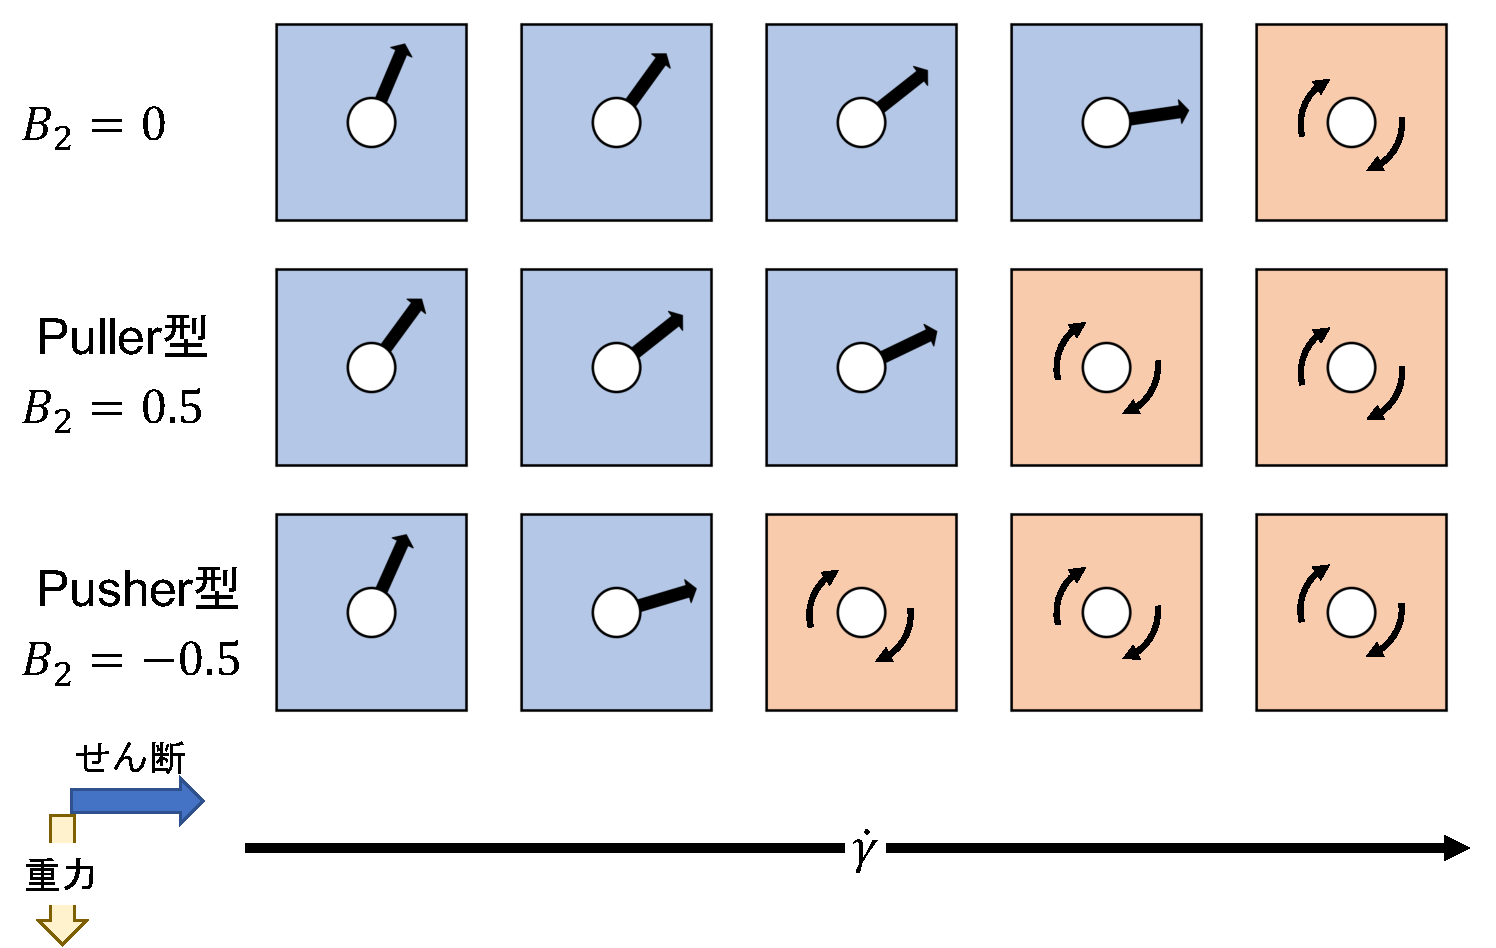
\includegraphics[scale=0.55]{/Users/taiga/Projects/lab/thesis/components/chapter4/figs/results.pdf}
        \caption{シミュレーションの模式図}
        \label{fig:results}
    \end{figure}

\noindent
上段は,通常の球形粒子にbottom heavy性を仮定したもの,
中段は,$B_2 = 0.5$のPuller型のsquirmer,
下段は,$B_2 = -0.5$のPusher型のsquirmerのシミュレーション結果である.
図中の直線の矢印は,定常せん断下での粒子の定常進行方向を表し,
曲がった矢印は粒子が定常回転していることを表す.
図の右側に行くにつれてせん断速度が大きいシミュレーションを表す.
また,左下に示したように,せん断は図の右向きに,
重力は図の下向きにかかっている.
この図より,せん断速度が小さい場合には,粒子はある進行方向に固定され,
粒子は回転せずに定常的にその方向に進むのに対し,
せん断速度が大きい場合には,定常的な回転運動を始めることが分かる.
これは,\ref{sec:rotation}で述べた予想に反しないと言うことができる.
